% Chapter 3
\newcommand{\voicescript}[0]{VoiceScript}
\chapter{Authoring Voice Recordings} % Chapter title
\label{ch:voicescript} % For referencing the chapter elsewhere, use \autoref{ch:mathtest}

%----------------------------------------------------------------------------------------
% Abstract
\begin{flushright}{\slshape    
The first sentence can't be written \\
until the final sentence is written.}\\ \medskip
--- \defcitealias{oates:1989}{Joyce Carol Oates}\citetalias{oates:1989} \citep{oates:1989}
\end{flushright}
%----------------------------------------------------------------------------------------
Speech recordings are central to modern media such as podcasts, audio books, e-lectures, and narrated documentaries. As with any serious authoring process, producing speech recordings involves an iterative back-and-forth between planning, authoring and editing. That is, producers repeat script writing, script editing, audio recording and audio editing back and forth multiple times. Throughout this process the script and the audio are closely linked to each other.\\

Yet, most existing tools treat the script and the audio separately, making the iterative workflow between them very tedious. Users have to switch between different applications to work on the script versus the audio, and manually translate edits in one mode to edits in the other mode. This process is especially time-consuming when there are multiple tracks involved, or when multiple people are collaborating on the same recording.\\

This chapter introduces \textbf{\voicescript}, an interface to support a dynamic workflow for script writing, audio recording and audio editing. \voicescript\ integrates the script with the audio such that, as the user writes the script or records speech, edits to the script are translated to the audio and vice versa.\\

We conduct informal user studies to demonstrate that our interface facilitates the audio authoring process in various scenarios. 
%
\section{Introduction}
Audio recordings of speech are prevalent across a variety of media, including podcasts, audio books, e-lectures and voice-overs for narrated videos.
%
Creating such audio recordings typically involves three main tasks: writing a script, recording the speech, and editing the recorded audio. 
%
While authors typically start by writing at least a rough script of what they plan to record, in practice, the process of creating the final audio rarely involves a simple linear progression through these steps. A more common workflow is to move back and forth between writing or editing the script, recording or improvising subsets of the speech, and editing together portions of multiple recorded takes.\\

For example, consider the case of recording the audio for an online lecture. After writing some notes to use as a rough script, the lecturer records a few takes and listens to the speech. She decides that one of the concepts requires a more detailed explanation, so she edits her notes, re-records the relevant speech, and merges the new recording into the final audio. Such updates may also happen in response to feedback from viewers after the lecture is published online. Similarly, when authoring a voice-over for a video, the initial recording may not align perfectly with the visual footage (e.g., some spoken explanations may be too short or too long for the corresponding video clips). In a collaborative scenario, an editor could request edits to the initial recording of a narrator. In each case, users may need to modify the script and re-record certain sections of the speech. In general, the process of recording and editing the speech together often reveals issues that require going back to edit portions of the script.\\

Unfortunately, most existing tools for authoring speech recordings do not facilitate this back and forth workflow. Typically, users write and edit the script in a text editing environment and then record and edit the audio in a different audio editing tool. The central issue  is that the written script and the recorded audio are treated as completely separate entities.
%
This separation introduces several sources of friction in the workflow. When the user records the speech, any deviations from the initial written text (either intentional or not) are not reflected in the script. Evaluating the recordings to decide what takes to choose or what script modifications are necessary requires careful scrubbing through the audio to find the relevant parts. In addition, once the user chooses a particular version of the speech to include, the script no longer matches the speech, which complicates any subsequent edits. Finally, if the user decides to modify a portion of the script, she must figure out what subset to re-record to ensure that the new recording can be merged in without creating audio artifacts (e.g., replacing a single word in a recorded sentence is hard to do since the word may not blend seamlessly with the adjacent words).\\

To address these challenges, we design \voicescript\, an interface that supports script writing, speech recording, and audio editing in a unified way. Our key idea is to maintain a so-called \textbf{master-script} that is linked to the audio and always reflects the current state of the project, including unrecorded, recorded, improvised and edited portions of the script. We use automatic speech recognition to transcribe the audio into text, and solve the task of combining together multiple recordings and syncing audio with the script like a text differencing and merging problem. To help users maintain a consistent master-script, \voicescript\ provides semi-automated tools for merging recorded takes into the master-script and visualizations that indicate what portions of the script need to be recorded or re-recorded in response to edits to the script. The combination of these features enables users to move back and forth between script editing, speech recording and audio editing in a seamless fashion.\\

\voicescript\ can be used to create audio recordings in a variety of workflows, including recording a fairly detailed script, recording without any script, and a collaborative scenario between two users. We conduct informal evaluations where users create their own audio recordings to summarize technical articles. We also compare \voicescript\ to a state-of-the-art text-based audio editing tool for the task of creating an audio recording from multiple raw recordings. The results demonstrate that \voicescript\ supports a wide range of workflows and enables first-time users to  easily author speech recordings. User feedback suggests that the integration of script and audio through the master-script greatly facilitates the authoring process. 

%----------------------------------------------------------------------------------------
\section{Previous Work}
\label{sec:voicescript_prevwork}
\subsection{Scripting}
Adobe Story \cite{adobestory2016}, FinalDraft \cite{finaldraft2016} and Celtx \cite{celtx2016} are examples of professional software dedicated to script writing. They support collaboration, automatic formatting, navigation and planning for future production, but they treat the script as a text document that is essentially separate from the recordings. In fact, in our formative interviews of lay and professional audio producers, we found that many of them use general-purpose document editors like Google Docs \cite{googledocs2016} or Microsoft Word \cite{microsoftword2016} to prepare their scripts.

\subsection{Recording and Editing Audio}
At the recording and editing stage, many users rely on commercial digital audio workstations, like Adobe Audition \cite{adobeaudition2016}, Avid ProTools \cite{avidprotools}, GarageBand \cite{garageband} and Audacity \cite{audacity}. Video editing software such as Adobe Premiere \cite{premier} or ScreenFlow \cite{screenflow} are also commonly used. These tools allow users to edit audio by manipulating waveforms in a multi-track timeline interface. They also provide a wide variety of low-level signal processing functions. However, since they are designed to serve as general-purpose audio production systems, they include many features that are not directly relevant for creating audio narratives whose main content is speech. Hindenburg Systems \cite{hindenburg} develops tools that are specifically targeted for audio narratives. Still, they are primarily concerned only with the audio and they do not deal with the script directly.   

\subsection{Text-Based Audio Editing}
Recently, several researchers have explored using audio transcripts to support text-based navigation and editing of audio. Whittaker and Amento \cite{whittaker2004semantic} demonstrate that users prefer editing voicemail through its transcript instead of its waveform. Inspired by similar intuition, Casares et al. \cite{casares2002simplifying} and Berthouzoz et al. \cite{berthouzoz2012tools} enable video navigation and editing through time-aligned transcripts. Rubin et al. \cite{rubin2013content} extend this approach to audio narratives and propagate edits in the transcript text to the corresponding speech track. These systems all focus on editing pre-recorded audio via its transcript, whereas we also consider how script edits influence the recording process and how audio edits also evolve the script. NarrationCoach developed by Rubin et al. \cite{rubin2015capture} also uses automatic speech recognition to align speech recordings with an input script. However, its focus, improving speech performance at recording time, is different from \voicescript. Here, we focus on facilitating the back-and-forth workflow between script writing and speech recording. \voicescript\ also takes advantage of text-based navigation and editing, but unlike these systems, it supports a dynamic workflow where both the audio recordings and the underlying script can be continuously updated.      

%----------------------------------------------------------------------------------------
\section{Design Principles}
To learn about current practices and challenges for creating speech recordings, we interviewed ten professional lecturers and two video producers who regularly create audio recordings for online lectures that are published on online platforms, including YouTube, Udacity, EdX and MITx. The following are several key insights we gained from the interviews.\\

\subsection*{Scripts are prevalent.} 
All of the lecturers prepared written materials about what they were going to say before they started recording. The format and level-of-details of these scripts varied. For instance, one lecturer used his lecture slides containing images and a list of bullet points as his script. Another lecturer typed a thorough word-for-word transcription of what he was going to say in a text document. Another person used handwritten notes as an outline. In all cases, while they were recording, they kept the scripts within their view and depended on them to guide their speech.  

\subsection*{Recordings deviate from the script.} 
In many cases, the initial scripts were rough or incomplete. Only two out of the ten lecturers we interviewed prepared a word-for-word script before recording. The majority used lecture slides or handwritten notes containing a rough outline of what they were going to record. They used these outlines as guides and improvised most of the actual recorded speech. One of the lecturers did an initial recording from the outline, and then used that to flesh out the script before recording additional takes. Even when a word-for-word script was prepared beforehand, the recording often did not follow the script exactly. While recording, the speaker sometimes remembered and added more details, or found a more natural way of saying a written sentence. In some cases, major script changes were made long after the initial recording was created. For example, one lecturer noted that he periodically revisited and re-recorded parts of lectures to add up-to-date examples. The result is that recorded speech almost always differs either slightly or significantly from the initial written script. \\

While a few people edited the written script to resolve these discrepancies, in most cases the script and recorded audio end up in inconsistent states. This inconsistency makes it difficult for users to update the recording. They cannot simply read and edit the script because it may not accurately represent the recorded audio. Moreover,  changing any portion of the recording requires identifying the appropriate subset of speech to re-record such that the new recording can be merged into the final track with no noticeable seams at the take boundaries.  

\subsection*{Final track includes multiple recordings.} 
As mentioned above, users almost always record multiple takes of the speech. Thus, assembling the final track typically requires merging these takes together using audio editing software. Many users noted that aligning the waveforms of multiple takes, finding the best take, and then cutting and joining them seamlessly were very time consuming and tedious tasks.

%----------------------------------------------------------------------------------------\
\section{The \voicescript\  Interface}
Based on these observations, we designed \voicescript , a speech authoring interface that supports script writing, speech recording and audio editing in a single unified workflow. Our interface is built on three key features.

\subsubsection{Text-based representation of audio.} 
We build on previous work~\cite{casares2002simplifying,whittaker2004semantic,berthouzoz2012tools,rubin2013content} that demonstrates the benefits of text-based representations of spoken audio for navigation and editing. \voicescript\ uses automatic speech recognition to transcribe audio recordings in realtime and represent each take with a verbatim transcript. As with previous systems, text edits to these transcripts are automatically propagated to the audio, which facilitates simple audio editing tasks. 

\subsubsection{Master-script view.} 
To help users manage the relationship between scripted text and recorded speech, we introduce the notion of a master-script that shows a unified view of both unrecorded portions of the script and recorded speech included in the final track. By representing and visualizing both recorded and unrecorded text, the master-script provides a complete, readable view of the current state of the project that evolves as the user records and adds new takes to the final track, edits recorded text, or modifies text that must be recorded. 

\subsubsection{Merge process.} 
Since recorded text typically differs from the script, \voicescript\ provides an interface for merging changes into the master-script. The fact that we represent all recorded audio as text allows us to use text differencing algorithms to identify conflicts and execute merges. One key difference between our scenario and standard text merging is that recorded audio cannot simply be cut and merged into the master-script at any arbitrary word boundary. In many cases, the temporal gap between spoken words is not big enough to produce a seamless edit in the final track. Our merge interface takes this into account and helps the user execute merges that are likely to be artifact-free.\\

The rest of this section describes our interface through typical usage scenarios of how users might create an audio recording. 
%
\subsection{Typical Usage Scenarios}
%
\begin{figure}
  \centering
  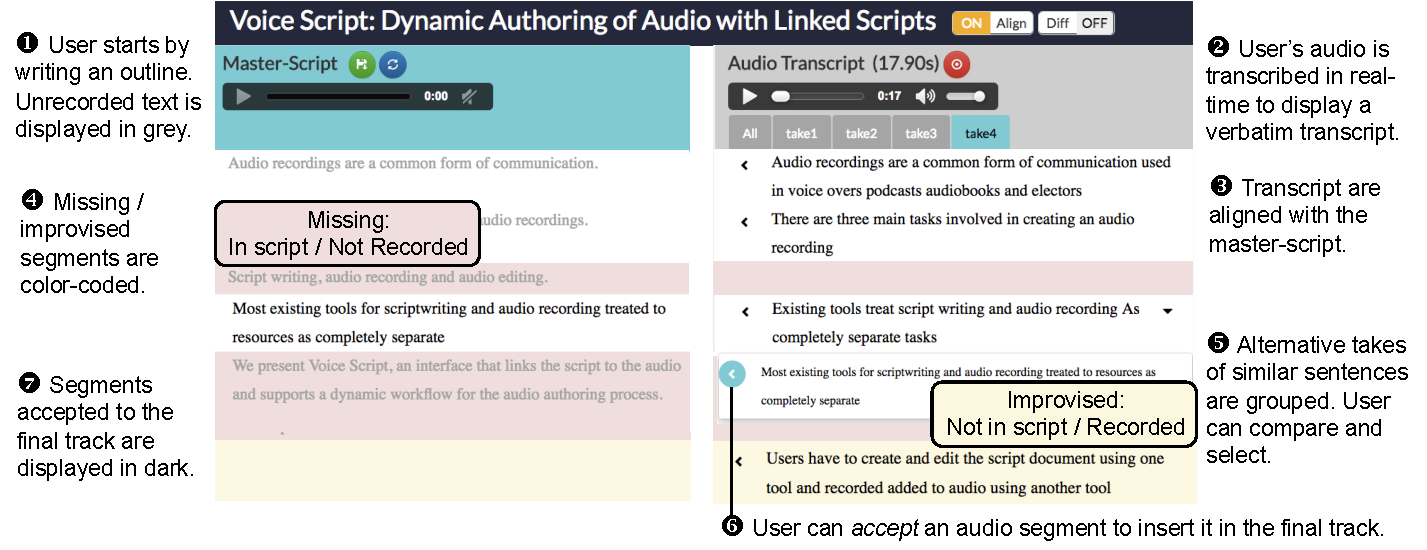
\includegraphics[width=\textwidth]{figures/ui_aligned2}
  \caption{The \voicescript\ interface. The master-script view on the left shows the current state of the project, including both recorded and unrecorded text. On the right, there are individual tabs for each recording, along with an 'All' tab that shows a summary of all takes.}~\label{fig:ui_aligned}
\end{figure}
%

\subsubsection{One-pass authoring.} 
Typically, the user begins by writing an outline of points to record in the master-script.
The text appears in light grey to indicate that these parts have not been recorded yet (Figure~\ref{fig:ui_aligned} \textit{left}). At this stage, the master-script is like an ordinary, editable text document. \\

Once the user starts recording, the audio is transcribed in real time and verbatim text corresponding to each take appears in a separate transcript tab (Figure~\ref{fig:ui_aligned} \textit{right}). Each transcript is time-aligned with the corresponding recording, so the user can quickly navigate to specific
parts of the audio by clicking on a word in the transcript. \\

The next task is to cut and merge parts of the recording into the final track. The user needs to compare the recording to the original outline, replace parts of the outline with the corresponding recording, and possibly insert improvised speech. To this end, we provide a \textbf{compare-view} that aligns segments of the recording transcript to corresponding segments in the master-script and shows them side-by-side. To indicate improvised portions of the audio, segments of the transcript that does not correspond to any part of the master-script are highlighted in yellow. To indicate missing portions in the audio, segments of the master-script that does not correspond to any part of the transcript are highlighted in red. To
view more detailed discrepancies between the script and recording, the
user can enable a \textbf{diff-view} that displays per-word differences
using standard track change markers, i.e., strikethroughs for
missing words and highlighting for added words (Figure~\ref{fig:diffview}).\\
%
\begin{figure}[!h]
\centering
  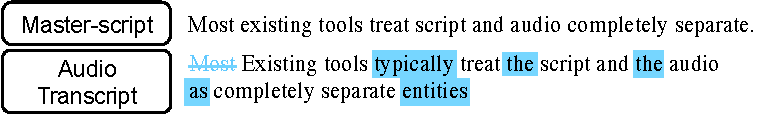
\includegraphics[width=0.8\columnwidth]{figures/diffview2.pdf}
  \caption{In the diff-view, users can view detailed, per-word discrepancies between the master-script and audio transcript.}~\label{fig:diffview}
\end{figure}
%

To add recorded audio to the final track, the user can \emph{accept} any portion of the recording by clicking a button next to the appropriate transcript segment. If there is a corresponding segment in the master-script, the accepted transcript segment replaces it. If there is no corresponding master-script segment, the accepted transcript segment is simply inserted into the master-script. Within the master-script, accepted segments appear in black to indicate that these are recorded portions of text that have been added to the final track (vs. grey for unrecorded text). \\

If there is more than one take, the user has to compare and select between multiple versions of the same segment. In addition to each of the transcript tabs, the \textbf{all tab} provides a summary of all of the takes. For each segment in the master script, this tab displays all the corresponding transcript segments from all of the audio takes. A drop-down button next to a transcript segment  indicates that there are multiple versions or takes of the  segment. Clicking on the button opens a list showing the alternative versions (Figure ~\ref{fig:ui_aligned}-5). The user can listen to any of these takes and select one without having to search through individual takes. \\

Finally, the user has to determine which parts of the outline is still missing. When the all tab is in focus, any part of the master-script that has not been recorded in any of the takes is highlighted in red. In this way, the user can tell at a glance what has already been recorded and what still needs to be recorded. All of the dark (i.e. recorded) text in the master-script represents the current state of the final audio track; all of the grey text has not been recorded or is recorded but the author has not yet accepted it into the final track. 

\subsubsection{Iterative and collaborative authoring.} 
The final recording is rarely produced in a single pass. Instead, the user often iterates back
and forth between editing the master-script, recording audio takes, and merging
audio segments into the final track. It is also common for multiple people to collaborate on a single voice-over. For example, a narrator who records the voice-over may work with others who write and edit the script, or several people may work on a recording with multiple voices. \\ 

During any point in the process, users can edit the master-script
like a text document.  For example, a user can simply insert
more text to record or make changes to unrecorded text to flesh
out the original outline. These edits can include verbatim script as well as comments or stage directions (e.g., "include examples" or "speak softer").
A user can also edit or delete recorded portions of the text. Deleting recorded text from the master-script will remove the corresponding portion of the audio from the final track. Altering recorded text can introduce audio artifacts (e.g., when a word is deleted mid-sentence), or it could mean that the corresponding text no longer matches the underlying audio. When the user edits a recorded word without completely deleting it, the word is flagged as \emph{dirty} (italicized and marked blue) to remind the user to review or re-record relevant portions. Finally, the user has an option to correct the transcription of recorded words without affecting the underlying audio or flagging it as dirty.\\

In both iterative and collaborative editing, users need to identify (1) new content that needs to be recorded for the first time, and (2) existing content that needs to be re-recorded after the script edits. To visualize this information, \voicescript\ keeps track of per-word metadata about whether a word is unrecorded (grey), recorded and unedited (black), or recorded and edited (blue italics). For collaboration, this metadata is passed between users with the script and recordings. The visualization and the text-based  editing and merging interface facilitate audio editing even when different persons work on different parts of editing the script, recording the audio and re-arranging the recorded audio. \\ 

\subsubsection{Other workflows.} 
One key benefit of our interface is that it supports a wide range of workflows for different users and scenarios. For instance, instead of starting with a written outline, the user can begin with an empty master-script, start recording, and then use the initial recording as an outline. The user can also record the entire script in a single take, or work on a single section at a time. \\

Please visit \url{https://people.csail.mit.edu/hishin/projects/voice_script/abstract.html} to see a video describing the interface. The voiceover for this video was created by two authors collaborating over \voicescript . We also look at various workflows in our informal user evaluation in Section~\ref{sec:usereval}. 

%----------------------------------------------------------------------------------------
\section{Algorithms}
\label{sec:algorithms}
Our authoring interface relies on audio transcription and text alignment algorithms to link the master-script to the audio recordings.  

\subsection{Transcribing the audio recording}
We use IBM Speech-to-Text Service \cite{ibmspeechtotext} to obtain a verbatim transcript of each audio recording in real-time. The service outputs a time stamp for each word indicating its start and end time within the audio. It also segments the transcript into \textit{utterances} where each utterance is separated by a longer silent gap in the speech (longer than 500 ms). While automatic speech recognition is imperfect, we have found that in most cases the results were accurate enough for the purpose of alignment (described below) and for users to understand the transcript. 
  
\subsection{Aligning the transcript to the master-script}
To support our side-by-side compare-view as well as the all tab view, we must identify corresponding parts of the master-script and recording transcripts. Moreover, we must partition these corresponding parts into segments that users can easily compare and merge into the master-script. Ideally, our segments should respect natural boundaries such as punctuations and line breaks in written text to aid readability. As discussed earlier, the segment boundaries should also align with longer pauses in the audio so that merge operations do not introduce obvious audio artifacts. Finally, we also want to separate parts of the transcript that generally agree with the master-script (i.e., planned speech) from parts that do not (i.e., improvised speech).  We designed a scoring function that optimizes for these requirements and use an iterative algorithm to co-segment the two texts. We first explain the algorithm and then describe the scoring function in detail.

\subsubsection{Iterative co-segmentation}
Before running our co-segmentation algorithm, we first compute the global word-to-word alignment between each recording transcript and the master-script using the Needleman-Wunsch (NW) algorithm \cite{needleman1970general}. NW allows for insertions and deletions, which account for differences in the two texts, for example, due to rough scripts, inaccurate speech, or transcription errors.\\

The segmentation of the master-script depends on the segmentation of the transcript and vice versa. Our iterative algorithm alternates between optimally segmenting the master-script and the transcript independently using the result from one to segment the other. We initialize the segment boundaries at punctuation marks (.!?:;) in the unrecorded text and silent gaps ($>$\ 500ms)\ in the recorded text. In practice, we
found that two iterations were sufficient to converge to a solution.\\

For each optimization step, we use the classic optimal line-breaking algorithm by Knuth and Plass \cite{knuth1981breaking}: The algorithm takes an input text $T$ and a reference text $R$, and outputs an optimal segmentation for $T$. Given the input text as a sequence of $n$ words $T = \{w_0,\dots,w_n\}$, the algorithm finds the optimal set of inter-word
boundaries that break the text into segments. We refer to the boundary between $w_i$ and $w_{i+1}$ as $b_i$.
%
The algorithm iterates through each word, and for each $w_i$
computes and records the optimal set of text segments $S_i$ for words up to $b_i$, along with the total score $E(S_i)$ of
this partial solution. $S_i =\{s_0, ... s_i\}$ is a sequence of segment labels, where $s_i$ is the index of the segment that word $w_i$ belongs to. To determine the optimal partial solution for $w_i$, it
considers each previous boundary $b_j$ $(j<i)$, and evaluates two possible ways of
segmenting the text $T_{ji} = \{w_\text{j+1},
\dots,w_\text{i}\}$: (1) appending $T_{ji}$ to the last segment in $S_j$, or (2) forming a new text segment with $T_{ji}$. The algorithm selects the better (lower) of the two scores for $T_{ji}$ and adds it
to $E(S_j)$ to obtain the total score for the proposed
segmentation. After considering all candidate boundaries $b_j$, the partial solution with the minimum segmentation score is stored as the optimal partial solution. Once the algorithm iterates through all the words, $S_n$ is the
optimal set of segments for the entire text $T$. 

\subsubsection{Scoring function}
The dynamic programming algorithm described above requires a
scoring function ($E$) that evaluates the goodness of a candidate segmentation. $E$ is a sum of the scores, $e$, for individual segments in the candidate segmentation. We define the scoring function
based on three terms: 
\begin{enumerate}
\item{\textit{Punctuation and silent gaps}: We prefer segment boundaries after sentence punctuation marks, and in case of recorded text, where there is a longer silent gap. Placing cuts at silent gaps allows audio segments from different takes or different parts of a single take to be joined seamlessly. More precisely, we define the boundary score, $e_b$, for a single text segment $T_{ji} = \{w_\text{j+1}
\dots,w_\text{i}\}$ as:
\begin{equation}
    e_b(T_{ji})= 
\begin{cases}
   1.0, \text{ if } w_i \text{ is unrecorded with punctuation (.!?:;)}\\
   -1.0 \text{ if } w_i \text{ is unrecorded without punctuation}\\
   t_{gap}(w_{i}) \text{ if } w_i \text{ is recorded} 
\end{cases}
\end{equation}

where $t_{gap}(w)$ is the silence gap in seconds after a recorded word, $w$, and is equal to 1.0 for $w$ that is at the end of a recording.
It is important to consider both the sentence punctuation and the silent gaps. As the examples in Figure~\ref{fig:scoringfunc} illustrate, considering only punctuation can result in audio artifacts when merging recordings. Similarly, considering only utterance boundaries can produce unnatural cuts in the middle of a scripted sentence.
}
%

\begin{figure}[!h]
\centering
  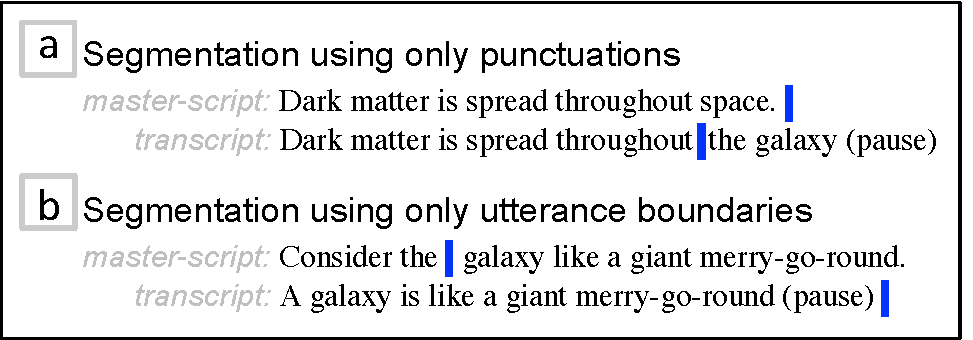
\includegraphics[width=0.8\textwidth]{figures/scoringfunc.pdf}
  \caption{Co-segmentation of master-script and transcript texts. (a) Segmentation using only punctuation marks results in abrupt cuts in the audio. (b) Segmentation using only utterance boundaries produces unnatural cuts in mid-sentence. Our scoring function takes into account both sentence punctuation marks and audio pauses.}~\label{fig:scoringfunc}
\end{figure}
%

\item{\textit{Global alignment}: We try to separate transcript segments that have a counterpart in the master-script (planned) from those that do not (improvised). Likewise, for the master-script, we want to separate segments that have a match in the transcript (recorded) from those that do not (unrecorded). We utilize the global alignment output from the Needleman-Wunsch (NW) algorithm. For each word $w_i$ in the input text, $T$, NW outputs a mapping 
to the reference text, $R$, and vice versa. For instance, $m_i$ is the index of the word in  $R$ that matches $w_i$. $m_i < 0$ if the word has no match. We prefer text segments that have the proportion of matching words close to 0 or 1. The alignment score, $e_a$, for a single text segment $T_{ji}$ is:  
\begin{equation}
e_{a}(T_{ji}) = 2\times\bigg|\sum_{n=j+1}^{i}{match(w_n)}\big/(i-j) - 1/2 \bigg|
\end{equation}
where $match(w_i)$ is 1 or 0, depending on whether $m_i \geq 0$ or not (whether the word has a match or not).
}
\item{\textit{Consistency with the other text}: Since the end goal is to align the segments from both texts, we would like the segment boundaries from the input text to align with the segment boundaries in the reference text even when the punctuation and utterance boundaries do not coincide. Let $S' = \{s'_0, \dots, s'_n\}$ be the segmentation of text $R$. Given this segmentation and the mapping of $T$ to $R$ from NW, the consistency score, $e_c$, for a text segment $T_{ji}$ is:
\begin{equation}
    e_c(T_{ji})= 
\begin{cases}
   1.0, \text{ if } s'_{m_i} \neq s'_{m_k} \text{ for the smallest } k>i, m_k \geq0\\
   -1.0 \text{ otherwise }
\end{cases}
\end{equation}

$s'_{m_i}$ is the index of the segment which $w'_{m_i}$ belongs to and likewise for $s'_{m_k}$. $w'_{m_k}$ is the closest word after $w'_{m_i}$ that has a match in $T$.
} 
\end{enumerate}

We combine these terms into a single scoring function $e$ as follows. 
\begin{equation}
e(T_{ji}) = e_a(T_{ji}) + e_b(T_{ji}) + 0.5  e_c(T_{ji})
\end{equation}
The goodness score for a set of text segments $S$ is:
\begin{equation}
E(S) = \sum_{T_{ji}\in S}{e(T_{ji})} - \big|S\big|
\end{equation}
where $\big|S\big|$ is the number of segments in $S$ and is a normalization term. For notational convenience, we use $T_{ji}\in S$ to refer to the set of contiguous words in $T$ that are assigned to the same segment in $S$. \\ 

We iteratively segment the master-script and the transcript texts. In practice, we found that 2 iterations was sufficient to converge to a final co-segmentation of the two texts.

\subsubsection{Alignment.} 
Given a co-segmentation of the master-script and the transcript text, we then compute the best matching master-script segment for each transcript segment. The match score between two text segments $T_1$ and $T_2$ is defined as the proportion of words in those segments that have a match between each other (from the NW output).
The result is an alignment between the master-script and transcript segments. 

We use this alignment to facilitate syncing and merging of script and audio by presenting tools similar to  common text differencing and merging tools. The compare-view displays matching segments side-by-side. Our color-coded visualization indicates which portions of the master-script is missing from the transcript, and which parts of the transcript are improvised (i.e., parts that do not have matching segments). In the all tab, segments from separate transcripts that match similar portions of the master-script are grouped together so that users can quickly compare and select between one of them. Similar to text or code merging, users can select a transcript segment to overwrite the matching master-script segment.



%----------------------------------------------------------------------------------------
\section{User Evaluation}
\label{sec:usereval}
\subsection{Informal User Study}
To assess the overall usability of \voicescript\ and to observe how users leverage various features of the interface, we conducted an informal evaluation with 4 users (U1-4). We started each session with a 10-minute demonstration of our interface. Then, we gave users a short article about a technical subject: \textit{What
is a Decibel?} from \url{howstuffworks.com} \cite{howstuffworks} or \textit{How Lasers Work} from
David Macaulay's illustrated book, \textit{The Way Things Work}
\cite{macaulay1999way}. The users' task was to create an explanatory audio recording about the subject using our interface. Users were allowed to refer to the article during the authoring process or to take notes on the master-script, but they were discouraged from recording the article by reading it out loud. We examined the users' workflow and solicited written qualitative feedback about the authoring experience at the end of the session. Each session lasted about 40 minutes.\\

While the size of our user evaluation is small, the initial findings are extremely encouraging. All users successfully produced a complete audio recording summarizing the article. %(Table 1). 

\subsubsection{\voicescript\ supports various workflows.} 
Interestingly, each user adapted a very different workflow. For example, U1 started by writing a complete list of main points. For each take, U1 recorded a few points from the list, merged them into the master-script, and then continued to record the next point on a separate take. In contrast, U2 wrote part of the script, recorded that portion, and moved on to write the script of the next part. U3 did not write an initial script, but improvised the recording and used that as a starting point to edit and re-record afterwards. Similar to U1, U4 started by writing a rough outline. But, instead of recording a few points, U4 recorded the full script at each take and merged the best parts to get the final track.\\

Sometimes users typed verbatim script to read aloud during the recording, and other times they wrote rough outlines. For example, U2 noted,  \textit{``For
the introduction, I had a pretty good idea of what I wanted to
say, so it saved me time to use only bullet points. [For the
second part] I wrote full sentences, as I was not familiar with
all the technical details and it would have been more difficult
to improvise. I enjoyed being able to use the master-script in
both ways.''}\\ 

The differences in the workflows could be due to personal preference, and/or  to the article content. In any case, our interface was able support various workflows. 

\subsubsection{The master-script facilitates iterative workflows.} 
As the above examples also demonstrate, users took advantage of the master-script to go back and forth between scripting and audio recording. For instance, U2 initially wrote a very rough outline for the script.
After recording and merging the first take based on this rough script, U2 refined the master-script, and then recorded more takes. Similarly, after recording and merging audio takes into the final track, U1 noticed a mistake in the speech
(i.e., instead of saying \textit{140 decibels}, U1 had said \textit{40}
decibels). U1 corrected the corresponding recorded text in the
master-script, re-recorded
the relevant portion part by reading out the edited master-script, and replaced it.
During the back-and-forth iteration, users took advantage of our color-coded visualization that indicated sections of the mater-script that required recording  (grey) or re-recording (blue italics). 

\subsubsection{Users found the master-script to be helpful.}
All users offered strong positive feedback about our authoring
interface, and said they would use it to create speech recordings. They were most enthusiastic about the integration
of the script and the recordings in the master-script document,
and the ability to align the master-script to the transcripts.
To quote from one user, \textit{``Writing the script on the same interface and having
that integrated with the audio was most helpful.''}  Another user noted
that the \textit{``compare-view helped to keep track of what pieces
of information was already recorded and which ones were still
needed.''} 

\subsubsection{Users were satisfied with the quality of the final recording.} 
Participants were satisfied with the overall quality
of the final recording. One user wrote, \textit{``I was surprised
how the final recording from the multiple takes was seamless.''} Users noted that while speech recognition was imperfect, \textit{``the transcriptions were accurate enough to understand and easy to check [by clicking to listen to the corresponding audio].''}

%------------------------------------------------------------------------
\subsection{Comparative study}

One of the main tasks in creating audio recordings is cutting and merging multiple audio takes. Many existing software specifically assist this task (see Section~\ref{sec:voicescript_prevwork} Previous Work). We separated out this audio editing task, and conducted a small comparative study to explore whether our master-script view facilitates the task compared to a state-of-the-art transcript-based speech editing interface \cite{rubin2013content}.\\
 
\begin{figure}[!h]
\centering
  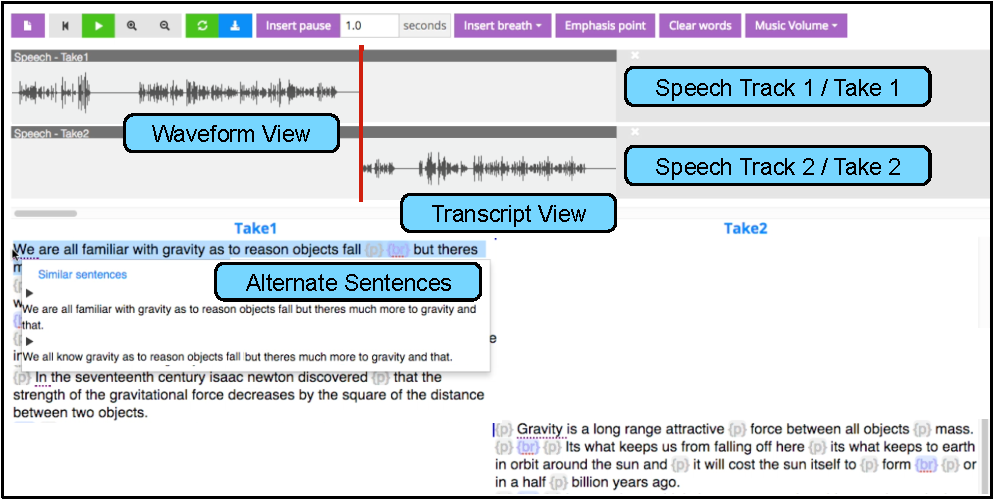
\includegraphics[width=1.0\columnwidth]{figures/interfaceR.pdf}
  \caption{Rubin et al.'s text-based audio editing tool (\textit{Interface-R}). For the purpose of our comparative study, each audio take was loaded as a separate speech track.}~\label{fig:interface-r}
\end{figure}

Similar to \voicescript , Rubin et al.'s interface (shown in Figure~\ref{fig:interface-r}, and referred to as
\textbf{Interface-R} hereafter) also uses time-aligned transcripts to support text-based editing. In both systems, users
can edit the transcript like a text document using operations
such as copy-and-paste, insert, or delete, and the edits are propagated
to the audio. Both systems also detect alternate takes of the
same sentence and groups them together so that users can easily compare and select between them.
However, unlike \voicescript , Interface-R does not have a master-script that integrates multiple audio recordings with a script. In fact, Interface-R does not explicitly handle multiple recordings. To simulate
multiple recorded takes, we took advantage of their multiple speech tracks,
so that each take appeared in a separate speech track (i.e., separate columns).\\

We recruited 4 participants, none of whom had
prior experience using text-based audio editing systems. We gave them
a script with bullet points outlining a mini lecture on a technical
subject (\textit{Gravity} and \textit{Dark matter}) and
two audio takes roughly corresponding to the script. In \voicescript , the script was contained in the initial master-script. Since Interface-R does not have a notion of
a script separate from the transcripts, we gave users a hard copy
of the script. The task
was to cut and merge the two pre-recorded takes to produce a recording that
contained all the contents listed in the script and only those
contents. The two takes were similar, but each take had some
missing content and some extra
content. The participants had to choose parts from each take
and combine them to get the final result. We encouraged the users
to focus on having the complete content rather than on the details
of the audio quality (e.g., tempo, diction, flow of speech).\\

Each participant completed the task twice, once on each interface using different scripts.
The subject of the lecture and the order of the interface were
counter-balanced. We examined the time users spent to complete the task, the number and type of functions they used, and the quality of the
final recording. After each task, participants gave written
qualitative feedback about their experience. In total, each session lasted about 1 hour. 

\subsubsection{Users completed the task faster using Voice Script.} All participants completed the task 25\% faster using our interface (average 7.4  vs 9.9 min), and also preferred it to Interface-R. The difference may be explained by the different workflow that each interface affords. In Interface-R, users effectively started with both recordings in the final track. They applied copy-and-paste to cut and merge the two takes, and deletion to remove redundant or superfluous content. In contrast, in \voicescript , users started with an empty final track. Then, using the compare-view, they accepted parts that matched the script from either of the takes. Although copy-and-paste and deletion were also available in \voicescript\ these operations were used only rarely, for example to delete a mistakenly accepted segment, to delete individual words, or to change the ordering of accepted segments (Table 1). \\
%
\begin{table}[!h]
\center
\tabcolsep3pt
\begin{tabular}{c|cccccc}
\multicolumn{7}{c}{\textbf{Audio Editing Session}}\\\hline
{User}&\multicolumn{2}{c}{Time spent}& {Total} & {Accept}
&{View}&{Text} \\
{}&\multicolumn{2}{c}{ours \textit{(Rubin)}}&{cuts}&{\textit{ind
/ all}}&{alternate}&{edit}
\\\hline
\textit{A}&\multicolumn{2}{c}{5:58 \textit{(08:10)}}&{3}& {4
/ 3}&{-}&{2}\\
\textit{B}  &\multicolumn{2}{c}{6:40 \textit{(11:10)}}&{3}&{3
/ 4}&{-}&{1}\\
\textit{C}&\multicolumn{2}{c}{9:37 \textit{(11:05)}}&{2}& {7
/ -}&{1}&{7}\\
\textit{D}&\multicolumn{2}{c}{7:25 \textit{(09:10)}}&{6}& {10
/ 1}&{3}&{-}
\\\hline
\end{tabular} 
\label{tab:editing}
\caption{Four participants created audio
recordings from two pre-recorded takes, using our interface and
Rubin et al.'s interface. Usage statistics pertain to our interface.
Accept \textit{ind / all} are number of segments accepted from
the individual transcript view and the \textit{all} tab view
respectively.}
\end{table} 
%
 %Each of the four participants preferred \voicescript\ over Interface-R %for the given task, and noted they would use
% our interface to edit audio recordings. Every participant also
% completed the task faster using our interface (7.4 $vs$ 9.9 min Interface-R). 
% Table 2 summarizes the participants' usage of our interface. Again users had different preferences for the individual transcript view and the \textit{all-tab} view. User B wrote,  \textit{``individual tabs were helpful after using the all-tab to make sure I hadn't missed content''} whereas user D \textit{``liked the individual tabs better since I wanted to view the original take as is.''} For this task, participants did not have to insert new content, but they used text editing operations to move content (e.g. copy \& paste)\ or delete portions of accepted segments from the final track.   

\subsubsection{The master-script facilitates merging.} 
Users appreciated having the master-script view. First, the master-script served to integrate the script outline and the recordings into a single comprehensive document. To quote from one user, \textit{``The master view integrated the two takes into an almost seamless whole that I just had to edit, as opposed to presenting two separate draft from which I had to generate a third and final story.''}  Secondly, the master-script helped users keep track of the status of the final track compared to the planned script. One user noted that \textit{``The outline [in the master-script] made it easier to find what I had accepted to the final track and what was still missing, instead of making notes on the paper outline and going back-and-forth between it and the recordings.'' } 

\subsubsection{The compare-view facilitates merging.}  
All 4 participants mentioned the align function in the compare-view as the most helpful feature in \voicescript . First, as one user noted, the segmentation in \textit{``the alignment view made editing much faster by visually breaking the script and the transcript into corresponding parts. I found I had to read much less.''} Also users found it \textit{``easier to click than to copy and paste''} in order to merge portions of recordings into the final track.  


%----------------------------------------------------------------------------------------
\section{Discussion}
\subsection{Limitations}
We rely on automatic speech recognition to transcribe the audio recordings in real time. Despite recent improvements in speech recognition \cite{hinton2012deep}, its performance varies widely. Transcription errors can affect the user's performance negatively (e.g., in navigating the audio, or if the user has to spend time correcting the errors) \cite{gaur2015effects}. In \voicescript , users can click on a word to listen to its corresponding audio and manually correct the transcription without affecting the audio. Taking advantage of the written script to fix or reduce speech recognition errors is an interesting area for future work.\\

\voicescript\ supports asynchronous collaboration to create voice recordings. Additional features are required in order to support synchronous collaboration, in particular, conflict resolution and version control.\\ 

Our interface focuses on the content of the speech recordings but does not consider editing details for audio quality. As one user mentioned in the feedback, we could integrate editing tools such as the ones in Rubin et al. \cite{rubin2013content} or \cite{rubin2015capture} to fine-tune audio quality. \\

Speech recordings often accompany visual footage or other sound effects such as music that is also closely related to the script/audio. Future work could investigate how to integrate these contents in the workflow.

\subsection{Conclusion}
To create speech recordings, people iterate back and forth between script writing or editing and audio recording or editing.  It is also common for several people to collaborate in the authoring workflow. Unfortunately, most existing tools treat the script and the audio as completely separate entities, which makes the dynamic workflow between them very tedious. We presented \voicescript , an authoring interface that facilitates iterative workflows for script writing and audio recording or editing. We used our system to collaborate asynchronously to create a voice-over. Through an informal user study, we demonstrated that our interface supports a wide range of workflows, and that our master-script seamlessly integrates scripting and recording. A comparative study showed that our system facilitates novice users editing speech recordings. 


